\chapter{Method}
\label{chap:method}
\textit{Using the information from \cref{chap:related work}, a proof of concept was designed where a step and heading system was combined with spatial context and activity recognition from IMU data from a smartwatch. This chapter begins with a design overview, whereafter each subsystem of the proof of concept and their respective components will be treated.}

\section{Proof of Concept System Overview}
The overall proof of concept, with all of its individual components, can be found in \cref{fig:system_design}. 
\begin{figure}[H]
	\centering
	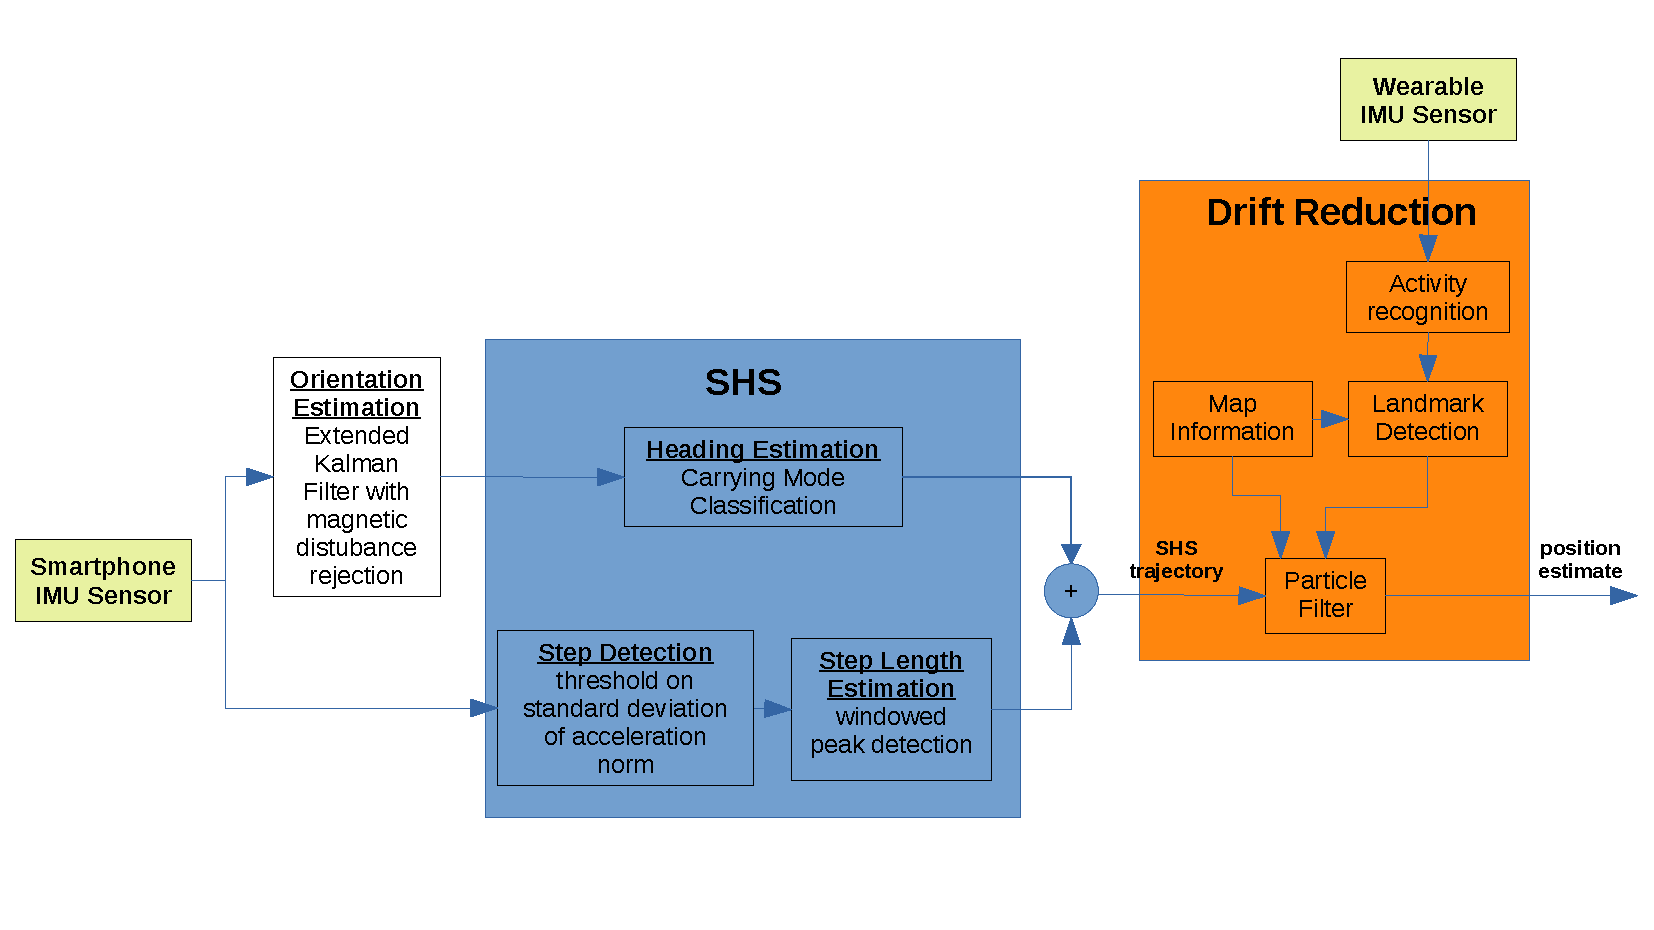
\includegraphics[trim=0 40 0 50, clip, width=1.1\linewidth]{images/system_design}
	\setlength{\abovecaptionskip}{3pt}

	\caption{Overview of Step and Heading System-Particle Filter (SHS-PF) proof of concept  with activity recognition from a smartwatch IMU.}
	\label{fig:system_design}
\end{figure}
The inputs to the system are map information and data from smartphone and smartwatch IMUs. The smartphone data will be used in a \ac{SHS}, outputting a trajectory walked. This trajectory will be used as the input for Particle Filter. The Particle Filter will also use map information and door interaction detection for measurement updates as a drift reduction method. The door interaction detection is activity recognition that uses thresholds on smartwatch IMU acceleration combined with standstill detection from the step detection component of the \ac{SHS}. 

\section{Smartphone based Step and Heading System}

In the following section the different components of the \ac{SHS}, indicated by the blue box in \cref{fig:system_design}, will be presented. The only input to this subsystem is the data from the smartphone IMU. The output is a trajectory consisting of connected step vectors,each with a step length and direction. The section will start with step detection, followed by step length estimation, heading estimation and drift reduction through a particle filter with spatial context.

\subsection{Step Detection}
\label{sec:meth - step detection}

Steps are reflected in accelerometer magnitude measurements by peaks in the trace. This caused by the impact of the foot with the ground. An extract of accelerometer magnitude data can be seen in \cref{fig:accelerometer_in_different_carrying_modes}. This figure shows how the accelerometer data changes per carrying mode. Peak detection can be used to extract the peaks from the accelerometer data. In \cref{sec:rw - step detection}, it was indicated that \citet{Brajdic2013} determined that windowed peak detection was a good approach in detecting steps from accelerometer data. \citet{Salvi2018} used this approach to optimize parameters for high performance step detection.

\begin{figure}[h]
	\centering
	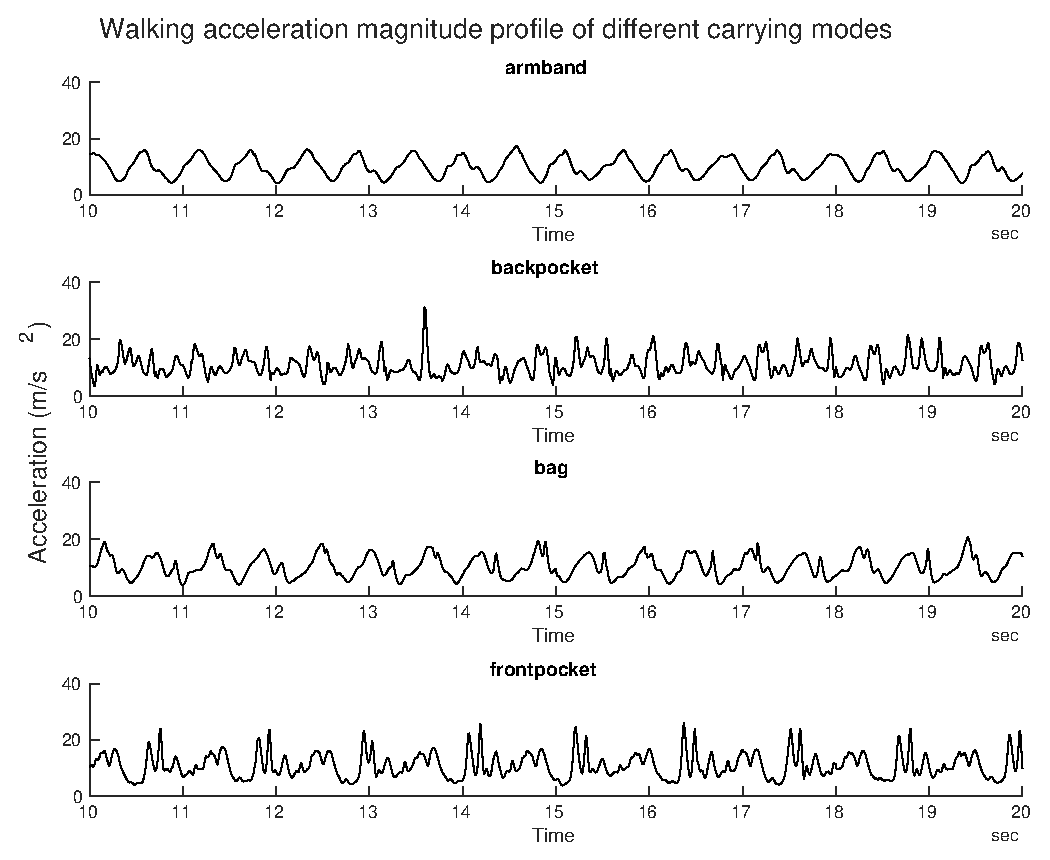
\includegraphics[width=0.8\linewidth]{images/20201127_1110__frontpocket_}
	\caption{Accelerometer magnitude in different smartphone carrying modes, showing difference in trace per carrying mode.}
	\label{fig:accelerometer_in_different_carrying_modes}
\end{figure}
 

The windowed peak detection method used in this thesis for step detection uses the implementation of \citet{Salvi2018}. The method consists of three stages applied to all \ac{IMU} accelerometer data, one after the other. \par  
The first stage of windowed peak detection consists of calculating the acceleration norm followed by the mean and standard deviation of the acceleration magnitude over a trailing moving window. All samples from this calculation with a standard deviation higher than a set threshold are considered walking and are used for further processing. The second technique is applying a Gaussina window function to the walk accelerometer magnitude data to smoothen it and amplifying peaks within the data using a score system. The third stage uses the output of the scoring technique to detect outliers, after which local maxima are flagged as steps.\par  

The thesis method augments the step detection method of \cite{Salvi2018} by adding the walk detection method from \cite{Brajdic2013}, since no formal walk detection was implemented in the original algorithm. This is used in order to filter out activities that are not walking, in an attempt to decrease the chance of false positives.\par 

The three stages used in step detection for this thesis will be handled in more detail next.

\subsubsection{Pre-processing and Walk Detection}
	 The \ac{IMU} used in smartphones provide acceleration information  $ y_a(k) \in \mathbb{R}^3 $ with a sampling frequency $ f $ and sample index $ k $, where $ k = 1,...,N $ where $ N $ is the total number of samples. For the first stage in step detection, the magnitude of acceleration from the three orthogonal axes is calculated 
			\begin{equation}\label{key}
		x(k) = ||y_a(k)||_2,
	\end{equation} 
	where $ x(k) $ now represents the accelerometer norm. \par 
	Since a person is not walking continuously, the time interval in which it does occur need to be detected. \citet{Brajdic2013} determined that thresholding on the standard deviation of the acceleration magnitude over a moving window was sufficient, using 
	
	\begin{subequations}	
		\begin{align}\label{key}
			x_{mean}(k) &= {\frac {1}{L_T f}}\left(\sum _{i=k-L_t f}^{k}{x(i)}\right)\\
			x_{\sigma}(k) &= {\sqrt {{\frac {1}{L_T f - 1}}\sum _{i=k-L_T f}^{k}\left(x(i)-{x_{mean}(k)}\right)^{2}}},
		\end{align}	
		\begin{align}\label{key}
			x_{walk}(k) &= 
			\begin{cases}
				x(k),& \text{if } x_\sigma(k)>A_{thres}\\
				Nan,              & \text{otherwise}
			\end{cases}
		\end{align}
	\end{subequations}
	Where $ x_{mean}(k)$ and $ x_{\sigma}(k) $ are the mean and standard deviation over the moving time window, where $ k = 1,...,N $. The time interval of the moving window is $ L_T $ in seconds and $ A_{thres}$ is the threshold on the moving window standard deviation. The samples who's calculated moving window standard deviation is above the prescribed threshold are considered walking and are passed to $ x_{walk}(k)$. For sample indexes where the threshold is not met, the value is indicated as not a number ($ Nan $). We perform the last step since $ x_{walk} $ will be used in the next stage of step detection, and we want to exclude the data below the threshold, but want to preserve the sample index over the whole dataset. Time will be preserved then as well. \par 
	
\subsubsection{Gaussian Window}
	In the second stage, a Gaussian window $ w(n) $ is applied to $ x_{walk} $ in order to smoothen the accelerometer magnitude \cite{Brajdic2013}, defined as
	
	\begin{subequations}
		\begin{equation}\label{key}
			w(n)=\exp \left(-{\frac {1}{2}}\left({\frac {n-{N_{filt}}-1/2}{\sigma_{gauss} {N_{filt}}-1/2}}\right)^{2}\right),
		\end{equation}
		where
		\begin{equation}
			n \in \mathbb{Z}, \quad 0\leq n\leq N_{filt}.
		\end{equation}
	
	Here  the window size is $ N_{filt} $ representing the number of samples in the window and $ \sigma_{gauss} $ the set standard deviation. The Gaussian window is applied to all the accelerometer data $ x_{walk} $, where $ k = 1,...,N $, through
	
	\begin{equation}\label{key}
		x_{gauss}(k) = \frac{\sum _{i=0}^{N_{filt}} x_{walk}(k-({N_{filt}}/2)+i)w(i)}{\sum _{i=0}^{N_{filt}} w(i)}.
	\end{equation}
	\end{subequations}
	
	

\subsubsection{Scoring and Outlier Detection}
	The result of the third stage uses a scoring calculation to increase the magnitude of peaks in the output of the Gaussian window stage, making it easier for the subsequent peak detection in the next stage.  The scoring used is that of mean difference, defined as 
	\begin{equation}
		x_{score}(k) = \frac{\sum^{N_{score}}_{i=-N_{score}, i \neq 0}\left(x_{gauss}(k)-x_{gauss}(k+i)\right)}{2 N_{score}}.
		\label{eq:mean difference}
	\end{equation}
	Here $N_{score}$ is the score window size in number of samples and $ k = 1,...,N $.\par 

	From this scoring output, outliers are statistically detected. The algorithm processes the signal by calculating a running mean and standard deviation as
	
		\begin{align}\label{key}
		x_{score, mean}(k) &= \frac{1}{k}\sum^{k-1}_{i=0}x_{score}(k-i),\\			
		x_{score,\sigma}(k) &= \sqrt{\frac{1}{k - 1}\sum _{i=1}^{k}\left(x_{score}(i)-x_{score, mean}(k)\right)^{2}}.
	\end{align}
	
	Using these two measures, statistical outliers can be determined. If the difference between the sample and mean is over a set threshold on the score standard deviation, then the acceleration magnitude is flagged as a potential step.
	
	\begin{equation}\label{key}
		x_{outlier}(k) = 
		\begin{cases}
			x(k),& \text{if } x_{score}(k)-x_{score, mean}(k)>B_{thres}x_{score, \sigma}(k)\\
			Nan,              & \text{otherwise}
		\end{cases}
	\end{equation}
	
	
\subsubsection{Step labeling}
	The final stage of step detection is determining local acceleration magnitude maxima of the outliers detected in the previous stage. Here local maxima are found using
	
	\begin{align}\label{key}
		i &= \in \mathbb{Z}, \\
		x_{step}(k) &= 
			\begin{cases}
			x(k),& \text{if } (\forall i \in (k-D_{step}f, k+D_{step}f)) \quad x(k)>x(i) \\
			Nan,              & \text{otherwise}
		\end{cases}
	\end{align}

	where maxima have a minimum separation duration between each other of $ D_{step} $ seconds.

\subsubsection{Parameters}
The parameters used from \citet{Salvi2018} are used. The researchers found these parameters through an exhaustive grid search across the parameter space. An overview of the values used can be found in \cref{tab:parameters_used}. 

\begin{table}[H]
	\centering
	\small
	\renewcommand{\arraystretch}{1.5}
	\begin{tabular}{llc} 
		\hline
		\textbf{Stage} & \textbf{Parameters} & \textbf{Value} \\ \hline
		\multirow{2}{*} {Threshold} & Acceleration standard deviation & $ A_{thres} = 0.6 m/s^2 $ \\
		& Frame length& $ L_T = $ 0.8 seconds\\
		\hline \multirow{2}{*}{Gaussian Window }& Window size & $\mathrm{N_{filt}}=13$ samples\\
		& Filter standard deviation & $ \sigma_{gauss}=0.35 $ \\ \hline
		\multirow{2}{25mm} {Scoring and Outlier Detection } 
		& Window size & $N_{score}=35$ samples\\
		 & Outlier threshold & $ B_{thres} = 1.1 x_{score,\sigma} $  \\ \hline 
		Step Labeling & Minimum separation duration & $D_{step} = 200 \mathrm{ms}$ \\
		\hline
	\end{tabular}
	\caption{\citet{Salvi2018} parameters used in thesis step detection stages.}
	\label{tab:parameters_used}
\end{table}

An example of the step detection method and its different stages can be found in \cref{fig:all_stages_of_step_detection}, where it has been applied to accelerometer data recorded during walking. The figure shows the working of each stage and how the peaks in the accelerometer data are determined.

\begin{figure}[H]
	\centering
	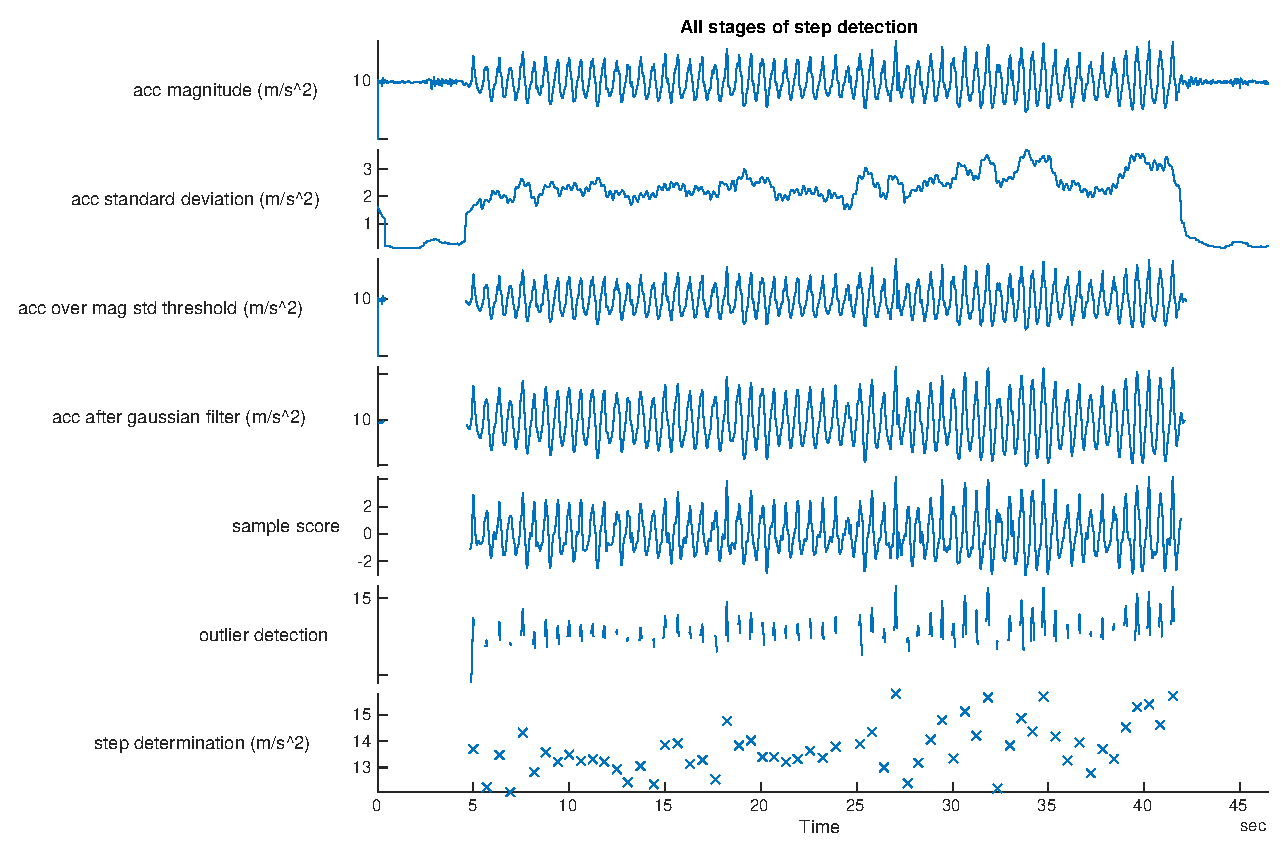
\includegraphics[width=1\linewidth]{images/20200924_1204_All_stages_of_step_detection}
	\caption[All stages of step detection ]{All stages of step detection from recorded accelerometer data, with the x's in the last graph indicating the accelerometer points that are flagged as being steps. }
	\label{fig:all_stages_of_step_detection}
\end{figure}

\subsection{Step Length Estimation}
For step length estimation the methods introduced in \cref{sec:step_length_estimation} using either global or personalized variables will be compared. These step length estimation methods require linear regression between their dependent variables and step length. All dependent variables can be distilled from accelerometer data and the output of the step detection component of the \ac{SHS}. \par 

In order to determine the linear relationships for the different models, accelerometer data recorded during walking is required where the traveled distance is known. Luckily, \cite{Vezocnik2019} have made the IMU data they used for their research available online under an open license. Running this data through the thesis step detection component, the result can be used for parameter estimation. Once the relevant parameters have been estimated, the performance of the methods can determined. This can be done by recording accelerometer data when walking, estimating the distance traveled using the step length methods and comparing it to the distance actually traveled.

\newpage
\subsection{Indoor Heading Estimation during Locomotion}

For heading estimation for the \ac{SHS}, the simplification was made to constrain the smartphone to one carrying mode, namely held in front of the body with screen pointing up, as shown in \cref{fig:experiment_carrying_position}. This was done because the unconstrained options outlined in \cref{sec:rw-step_heading_estimation} have low accuracy and detecting carrying mode through machine learning methods would add a complicated component to overall system. More importantly, the form of heading estimation does not directly help towards answering the research question of how activity recognition can help smartphone based indoor localization.\par 
\begin{figure}[H]
	\centering
	\includegraphics[width=0.4\linewidth]{images/IMG_4705}
	\caption{Smartphone carrying mode for indoor localization experiments with smartphone coordinate frame indicated by arrows.}
	\label{fig:experiment_carrying_position}
\end{figure}
%TODO write about euler angles
Through this simplification, the yaw orientation (euler angle rotation around the z axis in \cref{fig:experiment_carrying_position}) of the sensor directly reflects the heading estimate of the pedestrian. The Extended Kalman Filter introduced in \cref{sec:rw-orientation_estimation} will be used to estimate the orientation in quaternions, which can then be mapped into euler angles, of which yaw is one. \par 

Before orientation estimation occurs, the smartphone \ac{IMU} sensor will be calibrated using the method of \cref{sec:sensor_calibration}. This will need to be done in the indoor environment where the experiments will be performed, away from magnetic disturbances. The calibration will also need to be performed again if significant time has passed between calibration. If a difference of 30 minutes occurred, sensor calibration was performed.\par 

In \cref{sec:motion_and_measurement_models}, the orientation model in the EKF is defined using certain assumptions. These will need to be accommodated by the heading estimation algorithm.
The assumptions made by the orientation model  are that the gravity vector and a homogeneous magnetic field are dominant in the accelerometer and magnetometer readings, respectively. This is of importance with Pedestrian Dead Reckoning, as a walking motion will induce additional external forces caused by feet striking on the floor, affecting the acceleration measured by the IMU. Additionally, when localizing indoors, ferromagnetic structures within the built environment will affect the magnetometer readings \cite{Michel2015a}.\par 

In order to facilitate these assumptions, intervals will be applied to accelerometer and magnetometer readings. If the measurements fall within the interval only then will the appropriate measurement update occur. The use of these thresholds assumes that there will be periods during pedestrian locomotion in which the acceleration measured is that only of the gravity vector and magnetic field is only that of the homogeneous magnetic field within the indoor environment. \par 

The intervals for the accelerometer and magnetometer measurements were found empirically. For the accelerometer measurements a measurement update is performed if the accelerometer magnitude is between 10 and 9.6 $ m/s^2 $. For magnetometer measurements, the interval is set between 110\% and 90\% of the magnetic field strength found during sensor calibration in \cref{sec:sensor_calibration}. \par 

A practical aspect to consider is that sensor data from all IMU sensors does not arrive at the same time when recording. A measurement update or time update will be calculated depending on the information that is received. \par 

The resulting algorithm combines the EKF from \cref{sec:rw-EKF} with the above methods in \cref{algo:indoor_EKF}.

\newpage
\newgeometry{left=3cm,bottom=0.1cm}
\begin{algorithm}[H]
	\caption{Extended Kalman Filter for indoor orientation estimation}
	\label{algo:indoor_EKF}
	\SetAlgoLined
	\DontPrintSemicolon
	
	\KwIn{ \ac{IMU} data $y_{*,k}$ where * is either $ a, \omega \text{ or } m $ for either an accelerometer , gyroscope or magnetometer measurement. $ {k=1,..N}$  where $N$ is the total number of samples. Covariance matrices $\Sigma_{\omega}, \Sigma_{\mathrm{a}} $ and $\Sigma_{\mathrm{m}}$. }
	\KwOut{An estimate of the orientation $\hat{q}_{\text {k|k }}^{\text {nb}}$ and its covariance $P_{k | k}$ for $k=1, \ldots N$}
	
	
	\For{k = 1,...,N}{
		\If{$ y_{*,k}  $== $ y_{\omega,k} $}{
		\underline{Time update:}
		\begin{align}
			\hat{q}_{k | k-1}^{\mathrm{nb}}=\hat{q}_{k-1 | k-1}^{\mathrm{nb}} \odot \exp _{\mathrm{q}}\left(\frac{T}{2} y_{\omega, k-1}\right) \\
			P_{k | k-1}=F_{k-1} P_{k-1 | k-1} F_{k-1}^{\top}+G_{k-1} Q G_{k-1}^{\top}
		\end{align}
		with $Q = \Sigma_\omega$
	}
		
		\underline{measurement update:}\\
		\If{$ y_{*,k}  $== $ y_{a,k}$ and $ 9.6 m/s^2 <\norm{y_{a,k}} < 10 m/s^2 $ }{
		\begin{subequations}
			\begin{align}
				y_{k}&=
				y_{\mathrm{a}, k}, \\
				\hat{y}_{k | k-1}&=
				-\hat{R}_{k | k-1}^{\mathrm{bn}} g^{\mathrm{n}},\\
				H_{k}&=	-\left.\frac{\partial R_{k | k-1}^{\mathrm{bn}}}{\partial q_{k | k-1}^{\mathrm{nb}}}\right|_{{q_{k | k-1}^{\mathrm{nb}}}=\hat{q}_{k | k-1}^{\mathrm{nb}}} \quad g^{\mathrm{n}}.
			\end{align}
		\end{subequations}
	}
		\If{$ y_{*,k}  $== $ y_{m,k}$ and $ 0.9 \norm{y_{m,cal}} <\norm{y_{a,m}} < 1.1  \norm{y_{m,cal}} $}{
		\begin{subequations}
			\begin{align}
				y_{k}&=	y_{\mathrm{m}, k},\\
				\hat{y}_{k | k-1}&=	\hat{R}_{k | k-1}^{\mathrm{bn}} m^{\mathrm{n}},\\
				H_{k}&=	\left.\frac{\partial R_{k | k-1}^{\mathrm{bn}}}{\partial q_{k | k-1}^{\mathrm{nb}}}\right|_{{q_{k | k-1}^{\mathrm{nb}}}=\hat{q}_{k | k-1}^{\mathrm{nb}}} \quad m^{\mathrm{n}}.
			\end{align}
		\end{subequations}
	}
		\begin{subequations}
			\begin{align}
				\varepsilon_{k} &= y_{k}-\hat{y}_{k | k-1}\\
				\quad S_{k} &= H_{k} P_{k | k-1} H_{k}^{\top}+R \\
				\quad K_{k} &= P_{k | k-1} H_{k}^{\top} S_{k}^{-1}
			\end{align}
			
			
			\begin{align}
				\tilde{q}_{k | k}^{\mathrm{nb}} &=\hat{q}_{k | k-1}^{\mathrm{nb}}+K_{k} \varepsilon_{k} \\
				\tilde{P}_{k | k} &=P_{k | k-1}-K_{k} S_{k} K_{k}^{\top}
			\end{align}
			
		\end{subequations}		
		
		\underline{Renormalize the quaternion:}
		\begin{equation}
			\hat{q}_{k | k}^{\mathrm{nb}}=\frac{\tilde{q}_{k-1}^{\mathrm{nb}}}{\left\|\tilde{q}_{k | k}^{\mathrm{nb}}\right\|_{2}}
		\end{equation}		
	}	
\end{algorithm}
\restoregeometry
\section{Map based Particle Filter with Landmark Measurement Update}
\label{sec:method-particle_filter}
In \cref{sec:rw-drift_reduction}, the Particle Filter was introduced as a drift reduction method able to handle spatial context such as map information, landmarks and spatial models. In this section, the spatial information of the experimental setup is shown and the implementation of the specific Particle Filter components with \ac{SHS} input is presented. This implementation, together with the generic components outline in \cref{sec:rw-drift_reduction}, generates 
\cref{algo:bootstrap_PF}, summarizing the indoor localization Particle Filter approach.

\subsection{Map Creation}
In order to use spatial context with the Particle Filter, different sources were combined to generate a map of the experiment space. Rudimentary blueprints of the building were used to generate a diagram of the indoor environment, preserving the structure ratios. The positioning and size of furniture was estimated. The resulting image has clear color distinction between the different structures within the building, including walls, doors and furniture, as seen in \cref{fig:indoor_blueprint}. Through a comparison between structures in the generated image and satellite images, shown in \cref{fig:house_google_maps}, the image was transformed from pixel to meter coordinates. This provides the basis for incorporating spatial context within a Particle Filter.

\begin{figure}[H]
	\centering
	\begin{subfigure}[t]{.38\textwidth}
		\centering
		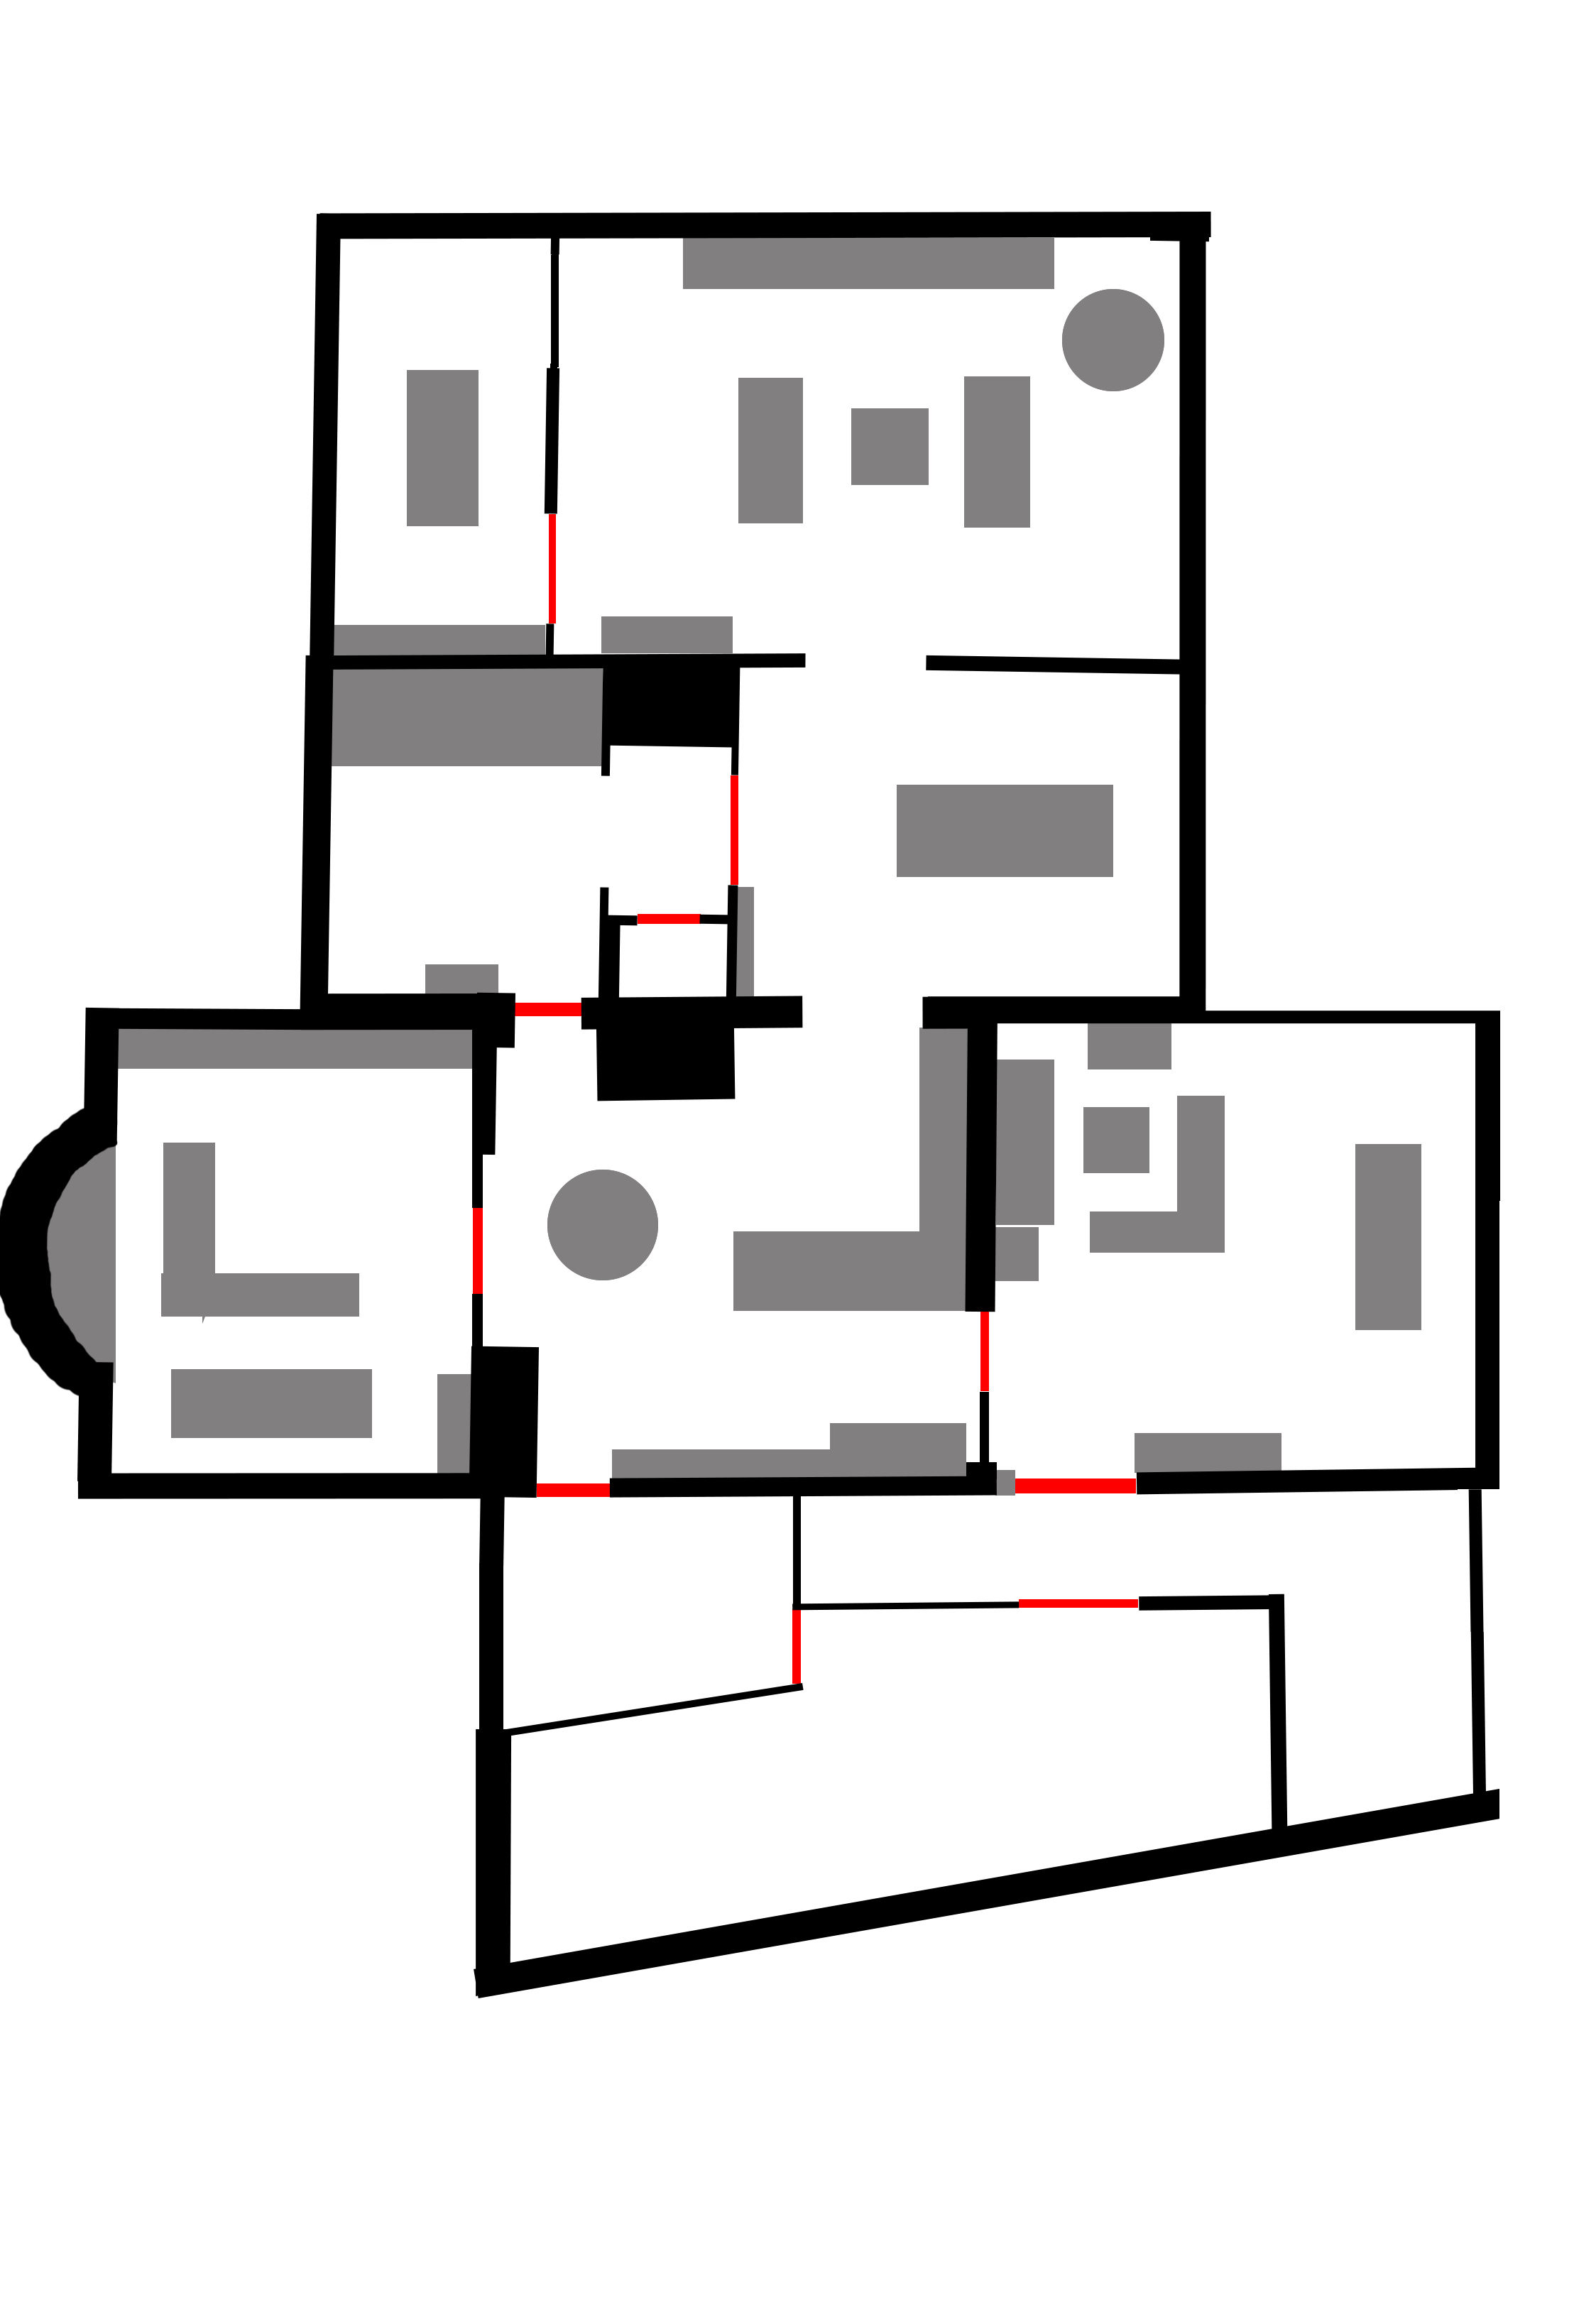
\includegraphics[width=0.9\linewidth]{images/indoor_blueprint}
		\setlength{\belowcaptionskip}{-5pt}
		\caption[Image from building blueprints]{Image from building blueprints. Black, grey and red represent walls, furniture, and doors, respectively.}
		\label{fig:indoor_blueprint}
	\end{subfigure} \quad
	\begin{subfigure}[t]{.4\textwidth}
		\centering
		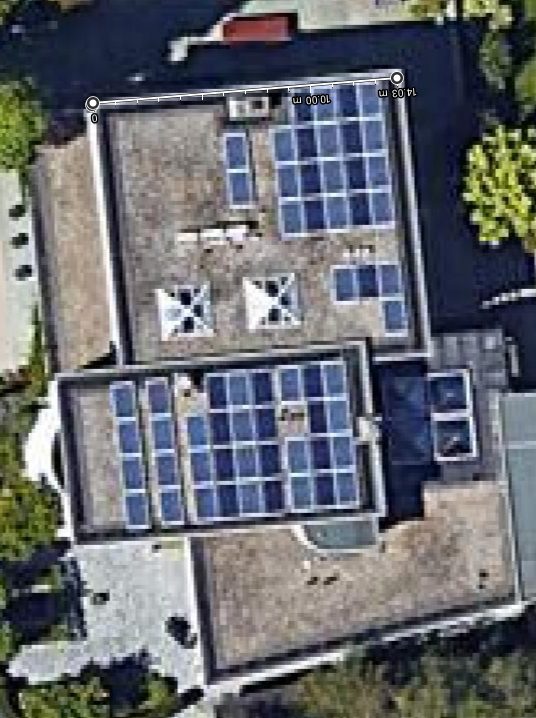
\includegraphics[width=0.9\linewidth]{images/house_google_maps}
		\caption{ Measurement from sattelite images. The red line indicates the measurement of 14.03 meters.}
		\label{fig:house_google_maps}
	\end{subfigure} \quad
	\label{fig:particle_map_construction}
		\setlength{\belowcaptionskip}{-20pt}
	\caption{Particle filter map creation from indoor blueprint and satellite image distance measurement}
\end{figure}

\subsection{State Representation and Initialization}
For indoor localization on one floor, particles are limited to $\mathbb{R}^{2}$ and by the outer perimeter of the building the user is located in. The particle is defined by 

\begin{equation}
\mathbf{x}_k^i = \left(\begin{array}{l}
	\mathbf{p}_{k}^i   \\
	\theta_k^i
\end{array}\right) = \left(\begin{array}{l}
p_{1,k}^i   \\
p_{2,k}^i  \\
\theta_k^i
\end{array}\right), 
\label{eq:pf_state}
\end{equation}
where $\mathbf{x}^i_k$ is the state of particle $i$ at time $k$, $\mathbf{p}_k$ is the position vector of the particle, where $p_1,k $ and $p_2,k$ are the particle x-axis and y-axis positions, respectively. The heading angle is  $\theta$. For initialization,  all particles are positioned around a known starting point. \par 

\subsection{Spatial Context Measurement Updates}
	There are two measurement updates used within the indoor localization Particle Filter, one that compares particle trajectories to map constraints and the other where door positions are compared with particle positions. \par 
	
	\underline{Spatial Constraints}\\
   With a map, the position of physical structures can be compared with the trajectory of particles as a measurement update. If these structures cannot be traversed, as is the case with walls, the trajectory of a particle that crosses such a structure is incorrect. This makes the likelihood of it being a position estimate 0, rendering its weight 0 as well. Particles that traverse accessible regions have a likelihood of 1, with all such particle receiving the same weight. This form of measurement turns wall information into a two dimensional probability density function ($p_{\scaleto{map}{4pt}}$). A grid based spatial model was used in which each pixel of \cref{fig:pf_map} that contained some form of obstruction was labeled as inaccessible for particles in the Particle Filter. The result is shown in \cref{fig:pf_map}, where black color regions are inaccessible and therefore have a likelihood of 0.\\
   Depending on this distribution, the individual particle weights are evaluated as 
   
   \begin{subequations}
   	\begin{equation}
   		\omega^i_{k|k} = \frac{1}{c_k} \omega^i_{k|k-1} p_{\scaleto{map}{4pt}}(\mathbf{x}^i_{k:k-1}),
   		\label{eq:pf_map_weight}	
   	\end{equation}
   	\begin{equation}
   		c_{k}=\sum_{i=1}^{N} w_{k | k-1}^{i} p_{\scaleto{map}{4pt}}\left( \mathbf{x}^i_{k:k-1}\right).
   		\label{eq:pf_map_normalization}
   	\end{equation}
   	\label{pf_map_update}
   \end{subequations}
   
   Here $x^i_{k:k-1}$ represent the individual particle path between its current and previous particle positions. This measurement update occurs every time step of the \ac{SHS}.   
   
   	\begin{figure}
   	\centering
   	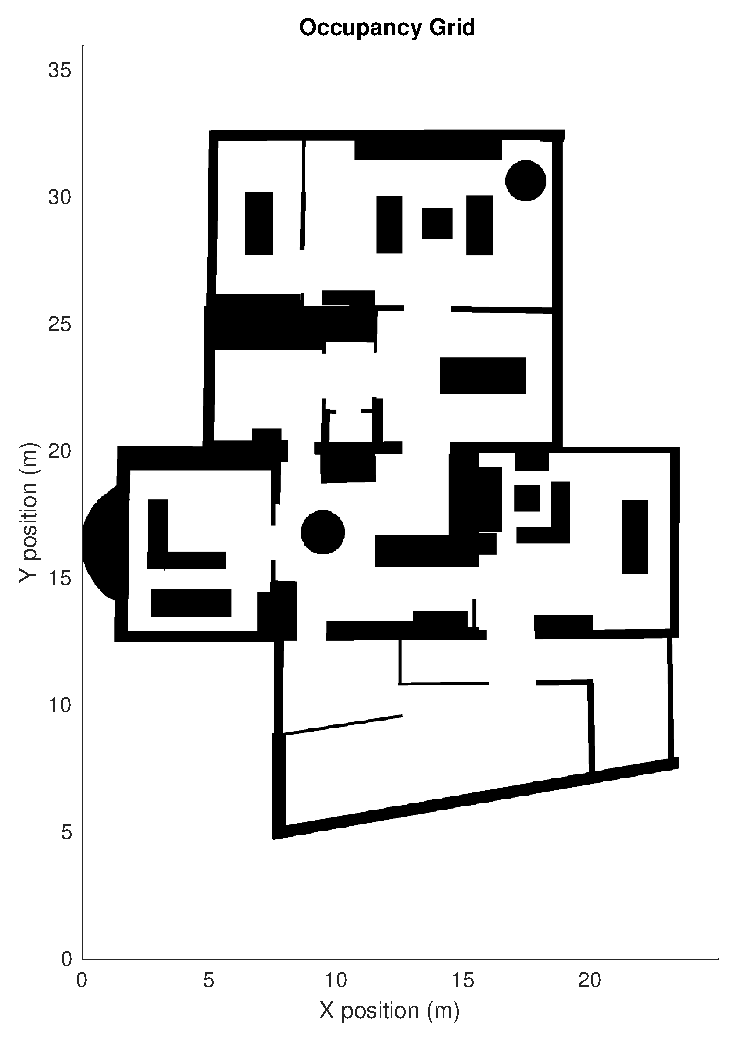
\includegraphics[width=0.4\linewidth]{images/20201030_1157_pf_map_1}
   	\caption{Particle Filter two-dimensional probability function, where white and black has a probability of 1 and 0, respectively.}
   	\label{fig:pf_map}
   \end{figure}
 
 		\underline{Door location}\\
	A map also indicates door locations, which are used as landmarks in the Particle Filter. Doors are used for landmark detection, since they are not easily detected from smartphones alone \cite{zhao2015lmdd}, but can potentially can be detect through a combination of smartphone and smartwatch. If a door opening is detected through activity recognition, a conditional probability at each particle can be used to determine its weight, as 
	\begin{subequations}
		\begin{equation}
			c^*_{k}=\sum_{i=1}^{N} w_{k | k}^{i} p_{\scaleto{door}{4pt}}\left(\mathbf{y}_{k} | \mathbf{x}_{k}^{i}\right)
			\label{eq:pf_door_normalization}
		\end{equation}
		\begin{equation}
			\omega^{i*}_{k|k} = \frac{1}{c^*_k} \omega^i_{k|k} p_{\scaleto{door}{4pt}}(\mathbf{y}_k|\mathbf{x}^i_k),
			\label{eq:pf_door_weight}	
		\end{equation}
	\end{subequations}

 where $\mathbf{y}_k$ is the position vector of the closest door to each particle, $w^i_{k|k}$ is the weight generated by the map constraint measurement update, and $w^{i*}_{k|k}$ is the new weight of particle $i$. The conditional probability function per particles is a bivariate normal distribution, shown in \cref{fig:pfdiagram}, and defined as 
 
 \begin{subequations}
 \begin{equation}
 p_{\scaleto{door}{4pt}}(\mathbf{y}_k|\mathbf{x}^i_k)={\frac {\exp \left(-{\frac {1}{2}}({ \mathbf{y}_k }-{\mathbf{p}^i_{k}})^{\mathrm {T} }{\boldsymbol {\Sigma }}^{-1}({ \mathbf{y}_k }-{\mathbf{p}^i_{k}}))\right)}{\sqrt {(2\pi )^{2}\mid {\boldsymbol {\Sigma }}|}}}
 \end{equation}
 
 where $ \mathbf{y}_k $ is the position vector of the closest door, and $ \mathbf{p}^i_{k} $ is the position vector of the particle $ i $. The covariance matrix $ \Sigma $ is defined as 
 
 \begin{equation}
 	\mathbf{\Sigma} =\left[ \begin{array}{ll}
 		\sigma_{\scaleto{door}{4pt}} & 0 \\
 		0 & \sigma_{\scaleto{door}{4pt}}
 	\end{array}\right]
 \end{equation}
\label{eq:pf_door_meas_update}
  \end{subequations}

 Where $ \sigma_{\scaleto{door}{4pt}} $ is the covariance along both axis of the bivariate distribution. This covariance is currently set at 0.1 meters, a value found empirically when testing the indoor localization particle filter.\par 
 
 The closest door to a particle is determined by the door location within the particle's conditional probability with the highest likelihood. This is directly correlated to the smallest distance between particle and door, as indicated by \eqref{eq:pf_door_meas_update}. In the case of \cref{fig:pfdiagram}, if a door activity is detected, the weight of particles P1 and P3 will be made higher than that of P2. \\
 This measurement update can only happen when a door interaction detection occurs, and always happens after the map constraint measurement update.
	
	\begin{figure}[]
			\centering
			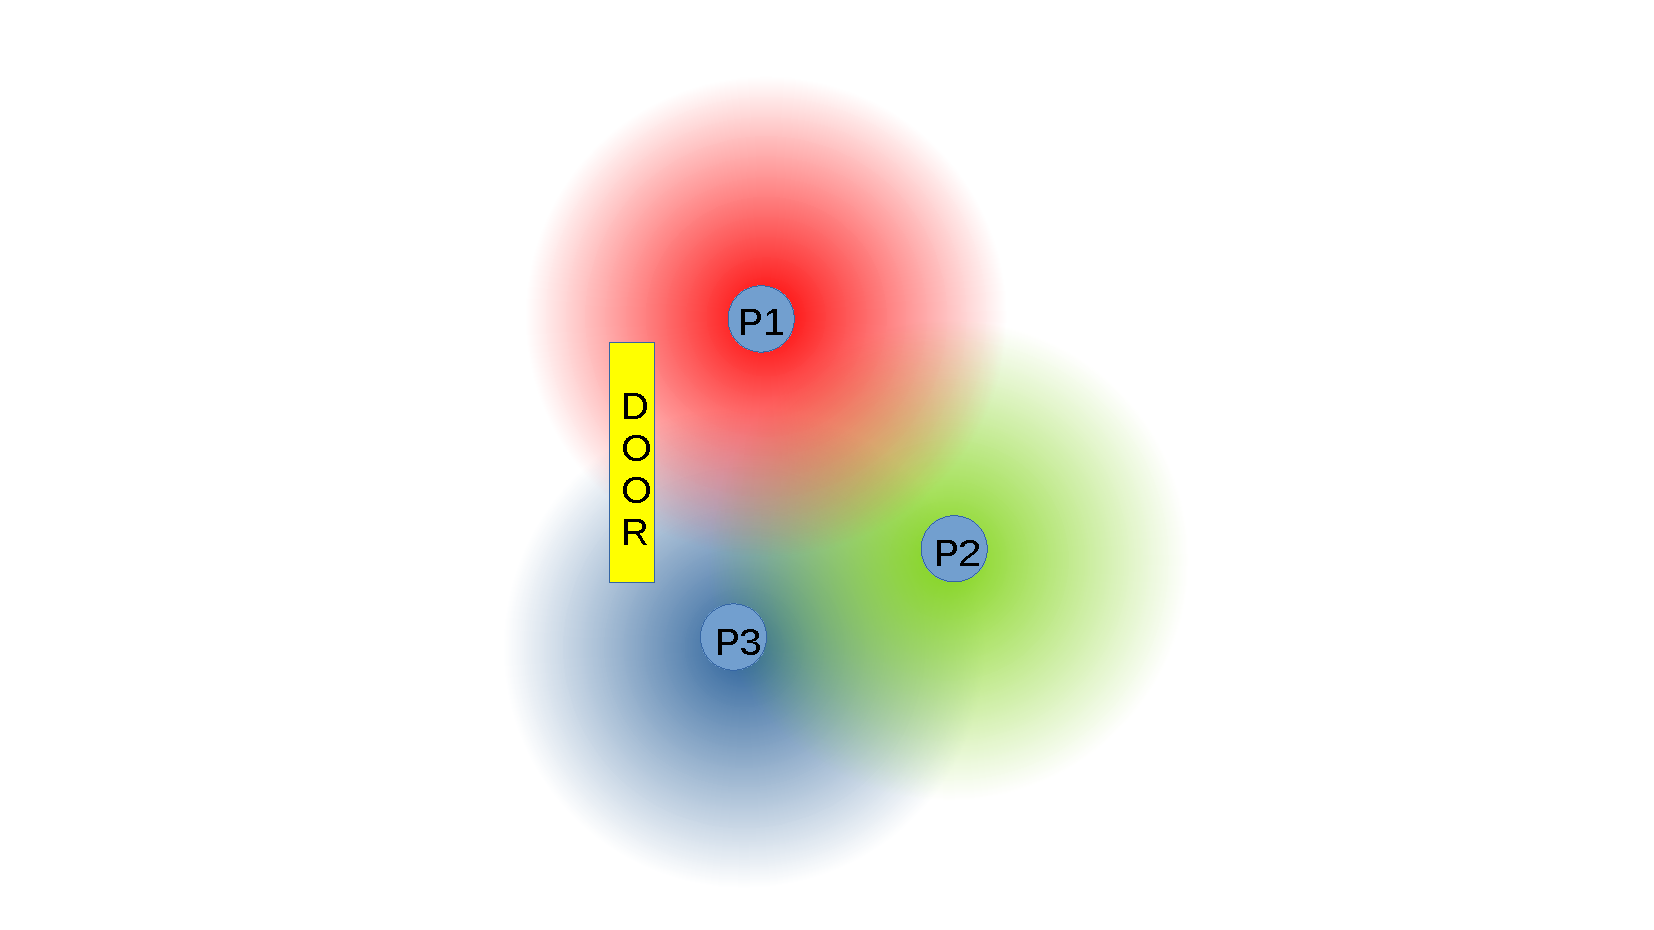
\includegraphics[trim=240 0 220 0, clip, width=0.35\linewidth]{images/pf_diagram}
			\caption{ Particles with a bivariate normal probability density function, represented by color gradient. At door interaction detection, particle weight is determined by probability at location of door in individual density functions.}
			\label{fig:pfdiagram}
	\end{figure}
	
	
\subsection{Step and Heading Time Update}
	After resampling, the new particles update their state with a dynamic model. For indoor localization using a step and heading trajectory as input, the dynamic model used is
	
	\begin{equation}
		\label{eq:SHS_dynamic_model_with_noise}
		\mathbf{x}^i_{k + 1}
		=
		\left(\begin{array}{l}
			p_{1,k}^i + (l_{k} + e_l) * \cos (\theta_{k}^i) \\
			p_{2,k}^i + (l_{t} + e_l) * \sin (\theta_{k}^i) \\
			\theta_{k}^i + \Delta \phi_k + e_\theta 
		\end{array}\right), \quad
		e_{\theta} \sim \mathcal{N}\left(0, \sigma_{\theta}^{2}\right), \quad e_{l} \sim \mathcal{N}\left(0, \sigma_{l}^{2}\right).
	\end{equation}

The inputs to this dynamic model are $l_{t}$ and $\Delta \phi_k$. The former is the step length found by step detection and step length estimation. The latter is the change in heading between the current and previous time step of the step and heading trajectory, found through the orientation estimation. These variables have additive zero mean Gaussian noise realizations $e_{\theta}$ and $e_{l}$, representing the uncertainty in the values of these inputs.\par 

The resulting Particle Filter from the previous steps is summarized in \cref{algo:bootstrap_PF}.
\newpage
\newgeometry{left=3cm,bottom=0.1cm}
\begin{algorithm}[]
	\SetAlgoLined
	\caption{Indoor Localization Particle Filter with Activity Recognition}
	\label{algo:bootstrap_PF}
	\KwIn{}
	\KwOut{}
	\underline{Initialization:}\\
	Choose the number of particles N.
	Generate initial distribution with
	\begin{subequations}
		\begin{equation}
		\mathbf{x}^i_1 \sim p_{x_1}, i = 1,...,N,
		\end{equation}
		and let
		\begin{equation}
			\omega^i_{1|0} = 1/N.
		\end{equation}
	\end{subequations}
	
	\For{k = 1,2,...}{
		\underline{Measurement update:}\\
		\begin{subequations}
			\begin{align}
				\omega^i_{k|k} &= \frac{1}{c_k} \omega^i_{k|k-1} p_{\scaleto{map}{4pt}}(\mathbf{x}^i_{k:k-1}),
				\label{eq:algo_pf_map_weight}\\	
				c_{k} &=\sum_{i=1}^{N} w_{k | k-1}^{i} p_{\scaleto{map}{4pt}}\left( \mathbf{x}^i_{k:k-1}\right)
				\label{eq:algo_pf_map_normalization}
			\end{align}
			\label{pf_map_update}
		\end{subequations}
		
		
		\begin{subequations}
			
			\If{(door interaction detected)}{
				\begin{align}
					c^*_{k}&=\sum_{i=1}^{N} w_{k | k}^{i} p_{\scaleto{door}{4pt}}\left(\mathbf{y}_{k} | \mathbf{x}_{k}^{i}\right)
					\label{eq:pf_door_normalization} \\			
					\omega^{i*}_{k|k} &= \frac{1}{c_k} \omega^i_{k|k} p_{\scaleto{door}{4pt}}(\mathbf{y}_k|\mathbf{x}^i_k),
					\label{eq:pf_door_weight}	
				\end{align}
			}
			\label{eq:pf_door_update}			
		\end{subequations}\smallskip
		
		
		\underline{Resampling:}\\
		\begin{subequations}
			\begin{equation}
				N_{\mathrm{eff}}=\frac{1}{\sum_{i=1}^{N}\left(w^{i}\right)^{2}},
			\end{equation}
			\If{	$N_{\mathrm{eff}} < 2N/3$}{
				
				\begin{align}
					x^{i*} &= x(F^{-1}(u^i)) \\
					u^i &= \frac{(i-1) + \tilde{u}}{N}, \tilde{u} \sim \mathcal{U}[0,1).\\
					\omega^i_{k+1|k} &= 1/N
				\end{align}
				
				\label{eq:pf_resampling}	
		}	\end{subequations}\smallskip
		\underline{Time update:}\\
		\begin{equation}
			\label{eq:algo_SHS_dynamic_model_with_noise}
			\mathbf{x}^i_{k + 1}
			=
			\left(\begin{array}{l}
				p_{1,k}^i + (l_{k} + e_l) * \cos (\theta_{k}^i) \\
				p_{2,k}^i + (l_{t} + e_l) * \sin (\theta_{k}^i) \\
				\theta_{k}^i + \Delta \phi + e_\theta 
			\end{array}\right), \quad
			e_{\theta} \sim \mathcal{N}\left(0, \sigma_{\theta}^{2}\right), \quad e_{l} \sim \mathcal{N}\left(0, \sigma_{l}^{2}\right).
		\end{equation}		
	}
\end{algorithm}
\restoregeometry
\newpage
\subsubsection{Indoor Location Estimation}
For the Particle Filter method outlined in this thesis, both minimum mean square error (MMSE) and maximum a posteriori (MAP) outline in \cref{sec:rw-pf} have disadvantages.
Firstly, MMSE does not work well in situations in which there are multiple equal likely hypotheses \cite{Saha2009}. In such a case it will take the position in between the different hypothesis as the position estimate. A good example of this can be found in \cref{fig:lopen_11_mmse_estimator}. The figure shows the output of a Particle Filter after 10 time steps. There are clear particle groups visible, all moving in different directions. The position estimate is expected to be in one of the particle clouds, however RMSE puts it between the different clouds, a position in which no particles are found, making it a subpar estimate. \par 
Implementing MAP as the state estimate in the Particle Filter is actually similar to MMSE. The measurement update that occurs every time step of the step and heading trajectory is the one that compares particle trajectories to map constraints. After this update all feasible particles will have the same weight. Since all particles have the same weight, a MAP cannot be defined. A MAP can only be defined sporadically when a door interaction measurement update occurs. 

\begin{figure}[H]
	\centering
	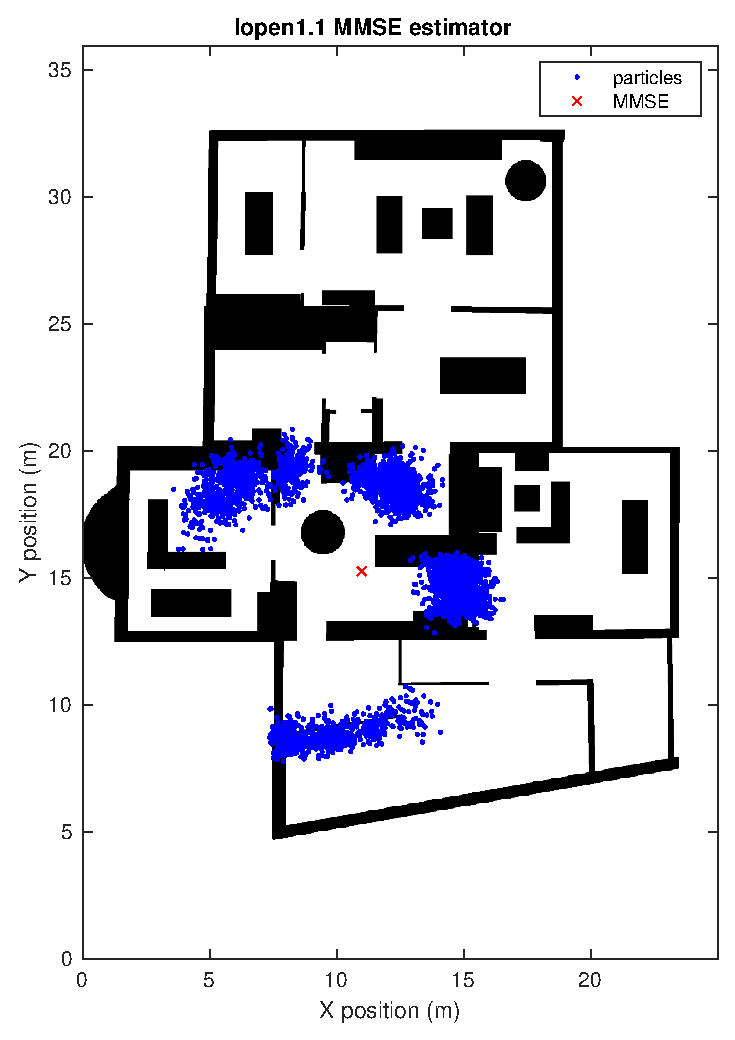
\includegraphics[width=0.35\linewidth]{images/20201108_1751_lopen1_1_MMSE_estimator}
	\caption{Particle filter after 10 iterations, showing how MMSE does not provide a suitable single point estimate.}
	\label{fig:lopen_11_mmse_estimator}
\end{figure}

The approach used for the indoor localization Particle Filter is to record the genealogy of particles, caused by resampling. Once the \ac{SHS} trajectory has been completed, the lineage of particles at the last time step are used to generate viable trajectories. Averaging the trajectories of multiple final particles is assumed to give an estimate trajectory within the indoor environment.
\newpage
\section{Door Interaction Activity Recognition}
\label{sec:method-AR}

In \cref{sec:method-particle_filter}, the Particle Filter is fashioned to use door interactions to perform a measurement update using spatial context. The door interaction is an activity that can be detected from smartwatch IMU data through activity recognition. \par 

Activity recognition is a large research field in which methods span a broad range of complexity, from simple thresholding to the use of deep learning techniques such as neural networks  \cite{Lima2019}. Even the subset of activity recognition that use \ac{IMU} sensors does not decrease the amount of possibilities significantly \cite{cornacchia2016survey}. The choice for a particular activity recognition method is often a trade-off between performance and computational complexity \cite{Bulling2014}. \par 

A smartwatch \ac{IMU} dataset was recorded in which interaction with door handle was indicated manually.
\cref{fig:smartwatch_acc_with_gt_door_and_door_detect} shows the smartphone accelerometer data for the three orthogonal axis. The vertical green and red lines indicating the start and end of the manually indicated interaction with a door handle, respectively. From this figure defining time domain characteristics can be spotted in the \ac{IMU} data when a door handle is being used. Within the door interaction intervals, the accelerometer signal clearly rises in the x-axis, with similar characteristics in the other axis.  Considering the scope of this thesis, where the goal is not focused on activity recognition, putting thresholds that encapsulate these characteristics is simple to implement and potentially sufficient in detect door interaction reliably.

\begin{figure}[H]
	\centering
	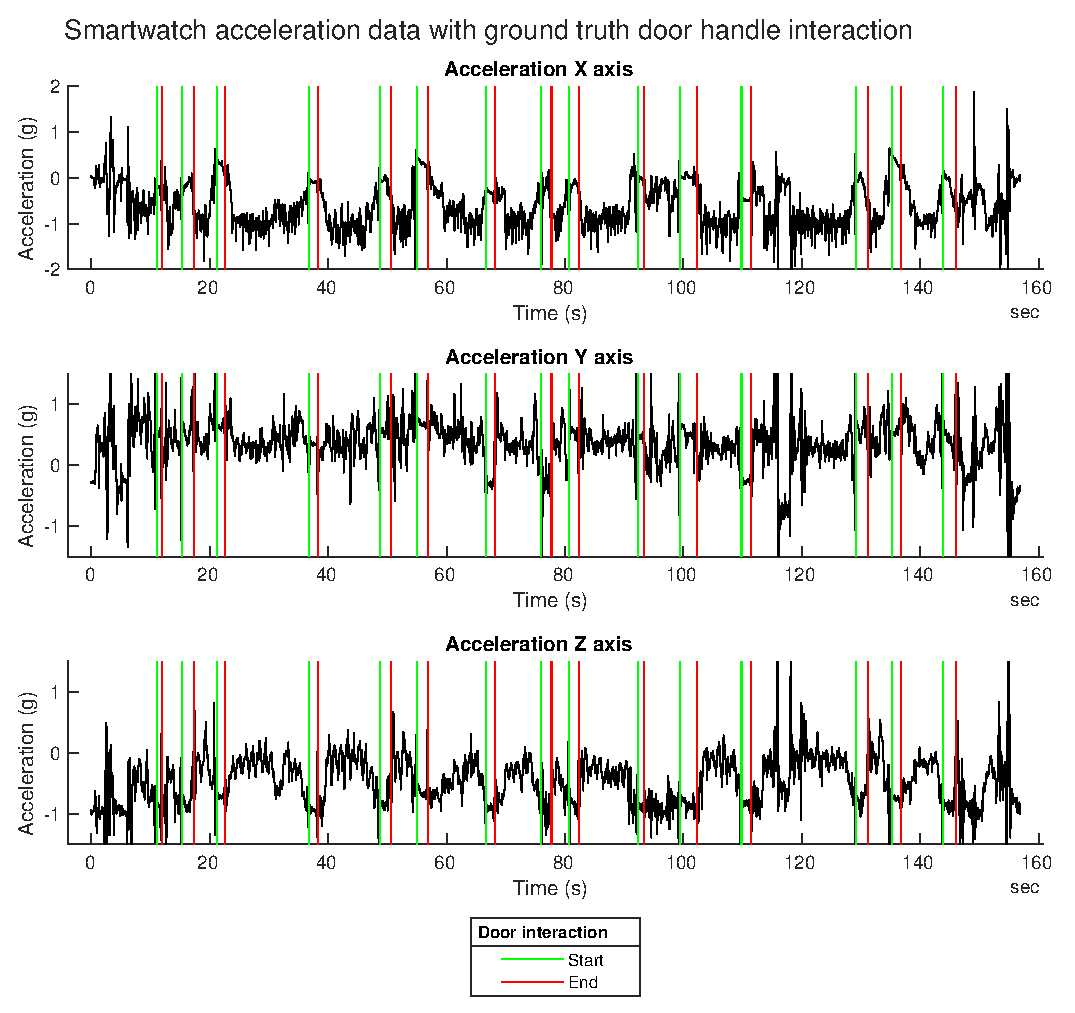
\includegraphics[width=0.8\linewidth]{images/20201123_1010_Acceleration_Z_axis}
	\setlength{\belowcaptionskip}{-20pt}
	\caption{Smartwatch accelerometer data with vertical green and red lines indicating start and end of manually indicated door handle interaction.}
	\label{fig:smartwatch_acc_with_gt_door_and_door_detect}
\end{figure}


\begin{figure}[H]
	\centering
	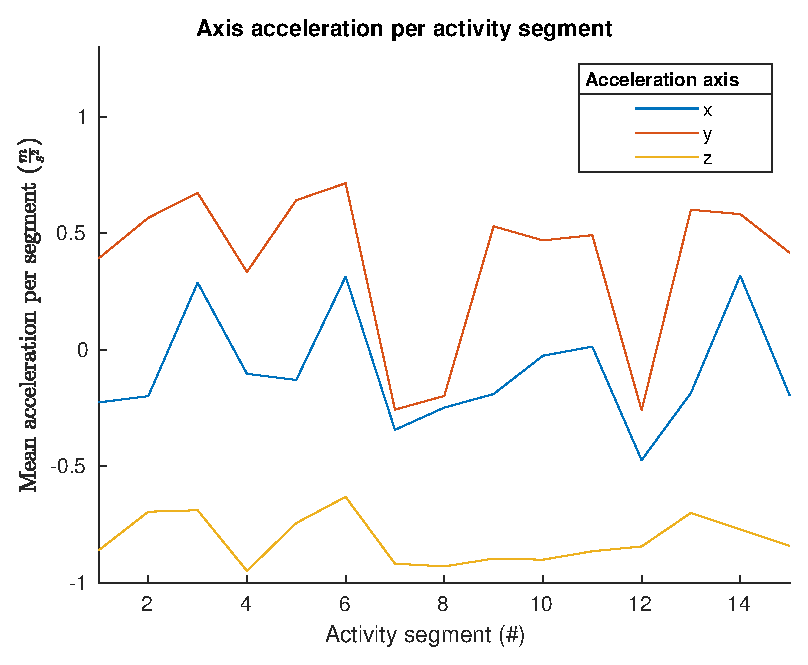
\includegraphics[width=0.6\linewidth]{images/20201114_1858_Axis_acceleration_per_activity_segment}
		\setlength{\belowcaptionskip}{-10pt}
	\caption{ Average accelerometer signal per axis of activity segments in \cref{fig:smartwatch_acc_with_gt_door_and_door_detect}, used to define thresholds for door interaction detection. }
	\label{fig:axis_acceleration_per_activity_segment}
\end{figure}

\begin{figure}[H]
	\centering
	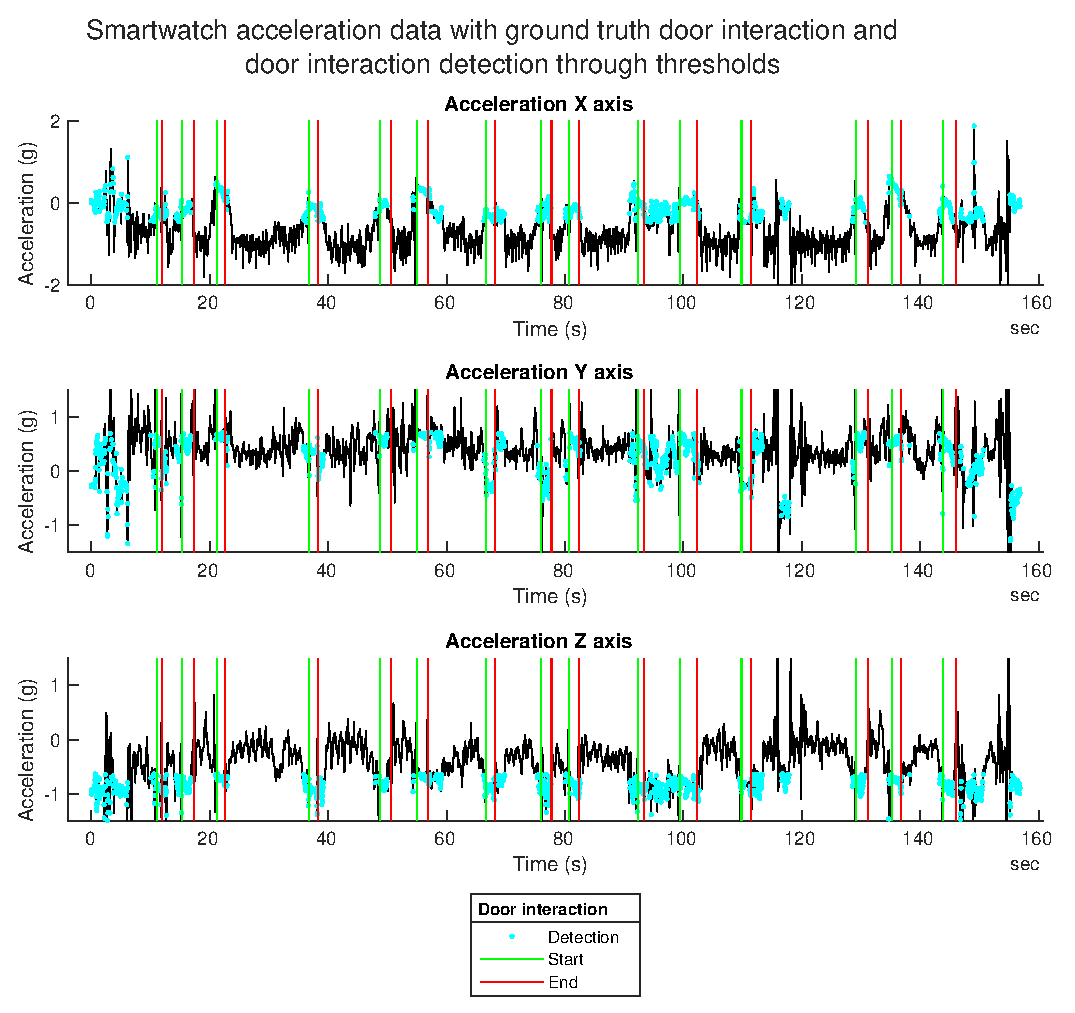
\includegraphics[width=0.8\linewidth]{images/20201123_1013_Acceleration_Z_axis}
	\caption{Smartwatch \ac{IMU} data with manually indicated door interactions and door interaction detections found through threshold defined in \cref{fig:axis_acceleration_per_activity_segment}}
	\label{fig:smart_watch_acc_with_gt_door_and_door_detect_2}
\end{figure}

\cref{fig:axis_acceleration_per_activity_segment} shows the average signal value for each accelerometer axis in each activity segment of \cref{fig:smartwatch_acc_with_gt_door_and_door_detect}. By taking the minimum of the x-axis mean and maximum of the y and z-axis mean from \cref{fig:axis_acceleration_per_activity_segment}, thresholds are defined.

In \cref{fig:smart_watch_acc_with_gt_door_and_door_detect_2} the thresholds are applied to the original data, presenting the performance of this approach. It shows the accelerometer data per axis, and the start and end of each activity segment. The cyan dots are samples that satisfy the activity thresholds defined before, and therefore represent door interaction detection. From this figure it shows that all activity segments have detection points, hence that threshold method is working. Unfortunately there are also detections not in activity segments, such as at 119 seconds. Such false positives will likely have an effect on the position estimate of the indoor localization Particle Filter, since it will trigger a landmark measurement update. This will unjustifiably increase the weight of particles close to doors, increasing the chance of them being resampling and potentially skewing the indoor localization estimate.  \par 

In an attempt to curb false positives, detections can be grouped in activity segments. Activity segments are defined by groups of detections that are below a set distance from their neighboring detections. This set distance is currently at 1 second. Segments that have less than 3 detections are disregarded. The start of a segment will be used for the door interaction measurement update in the indoor localization particle filter.\par

Another source of information that can help with the detection of door interaction originates from the \ac{SHS}. While interacting with a door, a pedestrian is often not taking any steps, something directly visible in the step detection component. An example of this can be found in \cref{fig:step_period_from_step_detection_while_walking_indoors}. Here the step period, which is the time between two detected steps, for a \ac{SHS} sample is shown. The green lines indicating the start of a door interaction, which were indicated manually. The plot shows that when interacting with a door, the step period increases for a short interval, since the pedestrian is standing still. Stationary intervals are detected by placing a threshold when step periods are above 1.5 seconds. This additional threshold can potentially help improve mitigating false positives, and will therefore also be used with the activity recognition scheme.

\begin{figure}[H]
	\centering
	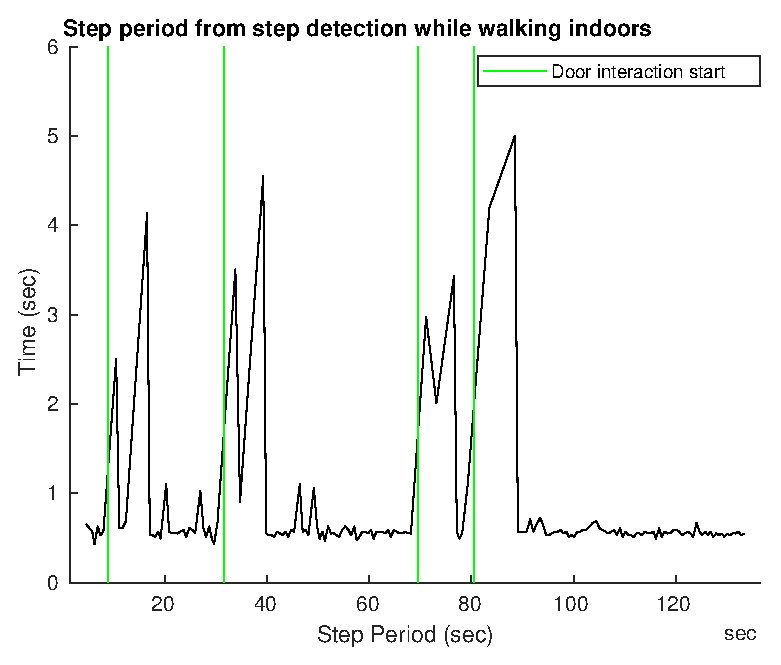
\includegraphics[width=0.55\linewidth]{images/20201122_1605_Step_period_from_step_detection_while_walking_indoors}
		\setlength{\belowcaptionskip}{-30pt}
	\caption{Step period while walking indoors with manually indicated start of door interactions. Data suggests that door interactions are often linked with temporary increases in step period.}
	\label{fig:step_period_from_step_detection_while_walking_indoors}
\end{figure}

